Dieser Abschnitt befasst sich mit der Kommunikation zwischen dem Client
und dem Server (z.B. Station auf der Erde und Rover auf dem Mars). Die
Kommunikation erfolgt hierbei {\"u}ber UDP Sockets. Das im verlauf der Arbeit
Implementierte CROP Protokoll verpackt zuvor die Inhalte (Bilder, Sensordaten etc.) 
nach den Protokollvorgaben und reicht die Datenpakete aus der priorisierten Queue 
direkt an den zuvor ge{\"o}ffneten UDP Socket weiter. Durch eine Client/Server
basierte Socket-Kommunikation {\"u}ber UDP 
(verbindungslose Kommunikation im Gegensatz zu TCP) wird der Datenstrom an die
definierte Zieladresse und den definierten Zielport geleitet. Da es sich
hierbei um eine UDP Socket-Verbindung handelt, werden Paketverluste nicht
bemerkt (keine Sicherung der Daten{\"u}bertragung). Lediglich ein {\"u}bergreifendes
Protokoll wie CROP, welches dies erkennen k{\"o}nnte, kann dann eine erneute
Sendung anfordern (zum jetzigen Zeitpunkt ist CROP jedoch nicht f{\"a}hig einen
Verbindungsabbruch zu detektieren). Die dabei genutzte Adressierungsart wird im
CROP Protokoll festgelegt und dann f{\"u}r die Socket-Kommunikation {\"u}bernommen. Im
Testszenario der Projektarbeit kam dabei IPv4 zum Einsatz.

\begin{figure}[H]
\centering
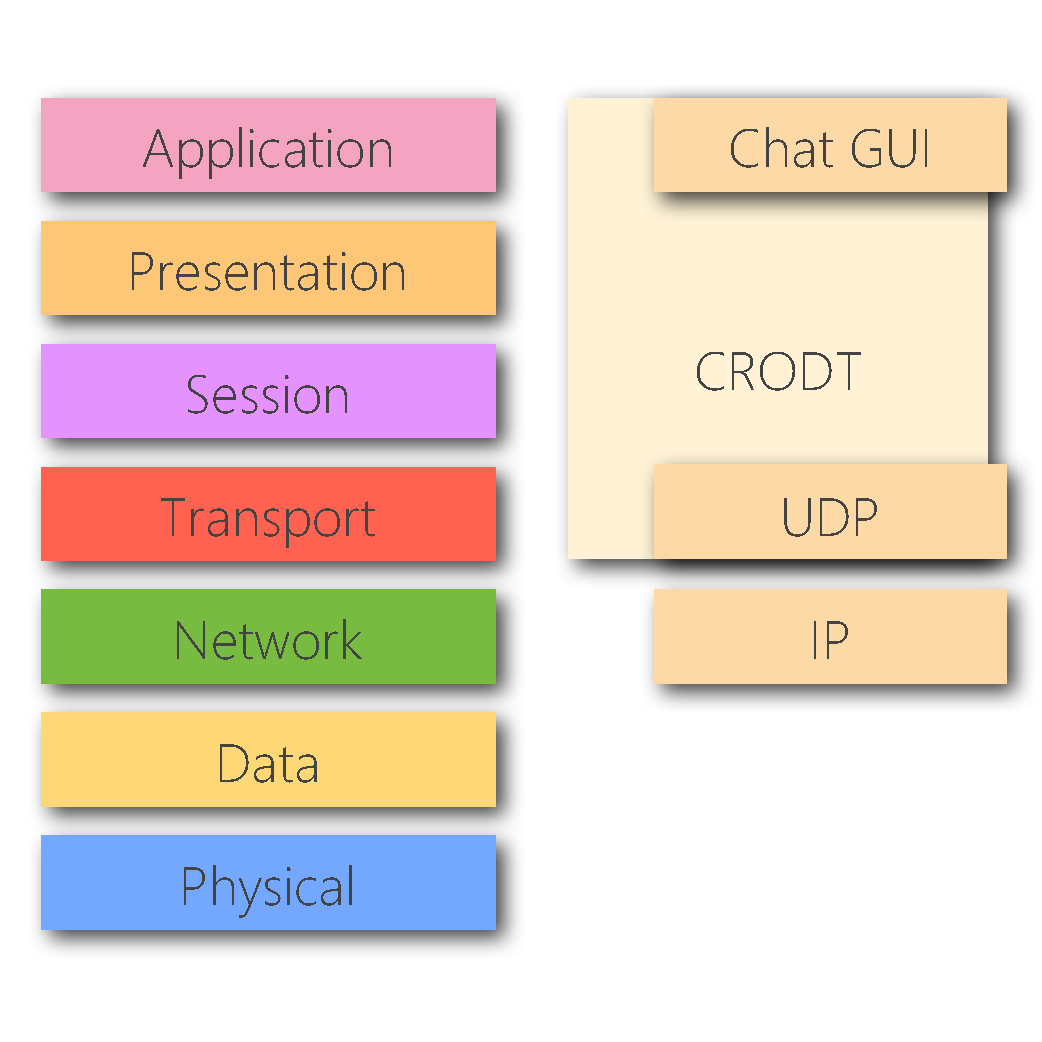
\includegraphics[scale=.38]{OSI.pdf}
\caption{{\"U}berblick des OSI-Schichtenmodells und der Zuordnung von CROP}
\label{fig:OSI}
\end{figure}